\documentclass[12pt]{article} 

\usepackage{amsmath,amssymb,amsfonts}
\usepackage{psfrag}
\usepackage{color}
\definecolor{darkblue}{rgb}{0.1,0.1,.7}
\usepackage[colorlinks, linkcolor=darkblue, citecolor=darkblue, urlcolor=darkblue, linktocpage]{hyperref} 
\usepackage[square, comma, compress,numbers]{natbib}
\usepackage[]{amsmath}
\usepackage[]{graphicx}
\usepackage[]{latexsym}
\usepackage{geometry}
\usepackage{amscd}
\usepackage[all,cmtip]{xy}
\usepackage{mathrsfs}
\usepackage[margin=10pt,font=small,labelfont=bf]{caption}
\geometry{verbose,letterpaper,tmargin=2.5cm,bmargin=2.5cm,lmargin=2.6cm,rmargin=2.6cm}
\usepackage{dsdshorthand}
\usepackage{changepage}
\usepackage{listings}
\setlength{\parskip}{0.1in}
\hyphenpenalty=1000

\numberwithin{equation}{section}

\renewcommand{\be}{\begin{eqnarray}}
\renewcommand{\ee}{\end{eqnarray}}
\newcommand\nn\nonumber 
\newcommand\cS{\mathcal{S}}
\newcommand\cR{\mathcal{R}}
\newcommand\SDPAGMP{\texttt{SDPA-GMP}}
\newcommand\SDPB{\texttt{SDPB}}
\newcommand\repl[1]{$\langle$\textrm{\em #1}$\rangle$}
\newcommand\defn[1]{\textrm{\em #1}\ $\equiv$}


\begin{document}

\noindent \today
\hfill {\em David Simmons-Duffin}
{\Large
\begin{center}
{\bf SDPB 1.0 \\\vspace{.1in}}
\end{center}
}
\tableofcontents

\section{Introduction}

\SDPB\ is an arbitrary-precision semidefinite program solver, specialized for ``polynomial matrix programs" (defined below).  This document describes \SDPB's usage and input/output.  Much more detail about its design is given in \cite{DSD}. The reader is encouraged to look there for a better understanding of \SDPB's parameters and internal operation.

\subsection{Installation and Requirements}

\SDPB\ requires

\begin{itemize}
\item \href{http://www.boost.org/}{The Boost C++ Libraries} (tested with Boost 1.54).

\item \href{https://gmplib.org/}{The GNU Multiprecision Library}.
\end{itemize}

To install, you must first edit the \texttt{Makefile} to define the variables
\texttt{GMPINCLUDEDIR}, \texttt{BOOSTINCLUDEDIR}, and \texttt{LIBDIR}. Then type \texttt{make} to
build the \texttt{sdpb} executable.

\section{Polynomial Matrix Programs}
\label{sec:PMP}

\SDPB\ solves the following type of problem, which we call a {\it polynomial matrix program} (PMP).  Consider a collection of symmetric polynomial matrices
\be
M_j^n(x) &=& \begin{pmatrix}
P_{j,11}^{n}(x) & \dots & P_{j,1m_j}^{n}(x)\\
\vdots & \ddots & \vdots\\
P_{j,m_j1}^{n}(x) & \dots & P^{n}_{j,m_jm_j}(x)
\end{pmatrix}
\ee
labeled by $0 \leq n \leq N$ and $1 \leq j \leq J$,
where each element $P_{j,rs}^{n}(x)$ is a polynomial in $x$.  
Given $b\in \R^N$, we would like to
\be
\label{eq:PMPconstraint}
\begin{array}{ll}
\textrm{maximize} & b_0+b\.y\quad\textrm{over}\quad y \in \R^N,\\
\textrm{such that} & M^0_j(x)+\sum_{n=1}^{N} y_n M^n_j(x) \succeq 0 \quad \textrm{for all $x\geq 0$ and $1 \leq j \leq J$}.
\end{array}
\ee
The notation $M\succeq 0$ means ``$M$ is positive semidefinite."



\section{Input to \SDPB}

\SDPB\ takes the following input:
\begin{itemize}
\item for each $j=1,\dots,J$:
\begin{itemize}
\item polynomial matrices $M^0_j(x),\dots,M^N_j(x)$ of maximum degree $d_j$,
\item bilinear bases $q_m^{(j)}(x)$ ($m=0,\dots,\lfloor d_j/2\rfloor$),
\item sample points $x_k^{(j)}$ ($k=0,\dots,d_j$),
\item sample scalings $s_k^{(j)}$ ($k=0,\dots,d_j$),
\end{itemize}
\item an objective function $b_0\in \R$ and $b\in \R^N$.
\end{itemize}
A bilinear basis is a collection of polynomials $q_m^{(j)}(x)$ such that $\deg q_m^{(j)} = m$, for example monomials $q_m^{(j)}(x)=x^m$.  (A better choice for numerical stability are usually orthogonal polynomials on the positive real line.)  The sample points and sample scalings determine how the PMP is represented internally as an SDP.  In principle, they don't affect the solution of the PMP, but in practice they can affect numerical stability.  The constant $b_0$ is completely irrelevant to the solution algorithm, but is included for convenience.  See \cite{DSD} for details.

\subsection{Input Format}

\SDPB\ reads the data above in the following XML format.

\begin{lstlisting}[
  caption={XML input format for \SDPB},
  label=xmlinputformat,
  mathescape,
  columns=fullflexible,
  frame=single,
  escapeinside=@@,
  basicstyle=\small\ttfamily\selectfont,
]
@\defn{input to \SDPB}@
  <sdp>
    @\repl{xml for objective}@
    @\repl{xml for polynomial vector matrices}@
  </sdp>

@\defn{xml for objective}@
  <objective>
    <elt>$b_0$</elt>
    ...
    <elt>$b_N$</elt>
  </objective>
  
@\defn{xml for polynomial vector matrices}@
  <polynomialVectorMatrices>
    @\repl{xml for polynomial vector matrix $M_1^n(x)$}@
    ...
    @\repl{xml for polynomial vector matrix $M_J^n(x)$}@
  </polynomialVectorMatrices>

@\defn{xml for polynomial vector matrix $M_j^n(x)$}@
  <polynomialVectorMatrix>
    <rows>$m_j$</rows>
    <cols>$m_j$</cols>
    <elements>
      @\repl{xml for polynomial vector $P^{n}_{j,11}(x)$}@
      ...
      @\repl{xml for polynomial vector $P^{n}_{j,m_j1}(x)$}@
      ...
      @\repl{xml for polynomial vector $P^{n}_{j,1m_j}(x)$}@
      ...
      @\repl{xml for polynomial vector $P^{n}_{j,m_jm_j}(x)$}@
    </elements>
    <samplePoints>
      <elt>$x_0^{(j)}$</elt>
      ...
      <elt>$x_{d_j}^{(j)}$</elt>
    </samplePoints>
    <sampleScalings>
      <elt>$s_0^{(j)}$</elt>
      ...
      <elt>$s_{d_j}^{(j)}$</elt>
    </sampleScalings>
    <bilinearBasis>
      @\repl{xml for polynomial $q_0^{(j)}(x)$}@
      ...
      @\repl{xml for polynomial $q_{\lfloor d_j/2\rfloor}^{(j)}(x)$}@
    </bilinearBasis>
  </polynomialVectorMatrix>

@\defn{xml for polynomial vector $P^{n}_{j,rs}(x)$}@
  <polynomialVector>
    @\repl{xml for polynomial $P^{0}_{j,rs}(x)$}@
    ...
    @\repl{xml for polynomial $P^{N}_{j,rs}(x)$}@
  </polynomialVector>

@\defn{xml for polynomial $a_0+a_1 x+\dots a_d x^d$}@
  <polynomial>
    <coeff>$a_0$</coeff>
    ...
    <coeff>$a_d$</coeff>
  </polynomial>
\end{lstlisting}

Several aspects of this format are inefficient.  Because the matrices are symmetric, \texttt{rows} and \texttt{cols} are redundant, and most elements are listed twice.  Also, XML is extremely verbose.  The current choices are in the interest of simplicity and could obviously be changed in a future version.

The options to \SDPB\ are described in detail in the help text, obtained by running ``\texttt{sdpb --help}."

\subsection{\texttt{Mathematica} Interface}

A \texttt{Mathematica} notebook \texttt{SDPB.m}, included in the source distribution, generates files of the form in listing~\ref{xmlinputformat} starting from \texttt{Mathematica} data.  It automatically makes sensible choices for the bilinear bases $q_m^{(j)}(x)$, the sample points $x_k^{(j)}$ and the sample scalings $s_k^{(j)}$.

The \texttt{Mathematica} definition of a PMP is slightly different but trivially equivalent to (\ref{eq:PMPconstraint}).  It is:
\be
\label{eq:PMPconstraintMathematica}
\begin{array}{ll}
\textrm{maximize} & a\.z\quad\textrm{over}\quad z \in \R^{N+1},\\
\textrm{such that} & \sum_{n=0}^{N} z_n W^n_j(x) \succeq 0 \quad \textrm{for all $x\geq 0$ and $1 \leq j \leq J$},\\
 & n\.z = 1.
\end{array}
\ee
where $W_j^n(x)$ are matrix polynomials.  The normalization condition $n\.z=1$ can be used to solve for one of the components of $z$ in terms of the others.  Calling the remaining components $y\in \R^N$, we arrive at (\ref{eq:PMPconstraint}), where $M_j^n(x)$ are linear combinations of $W^n_j(x)$ and $b_0,b_n$ are linear combinations of the $a_n$.  This difference in convention is for convenient use in the conformal bootstrap.

\texttt{SDPB.m} defines a function \texttt{WriteBootstrapSDP[file, sdp]}, where \texttt{file} is the XML file to be written to, and \texttt{sdp} has the following form, where the polynomials $Q^n_{j,rs}(x)$ are the elements of $W_j^n(x)$.

\begin{lstlisting}[
  caption={Usage of \texttt{WriteBootstrapSDP} in \texttt{SDPB.m}},
  mathescape,
  columns=fullflexible,
  frame=single,
  escapeinside=@@,
  basicstyle=\small\ttfamily\selectfont,
]
@\defn{function call}@ WriteBootstrapSDP[file, @\repl{sdp}@]

@\defn{sdp}@ SDP[@\repl{objective}@, @\repl{normalization}@, @\repl{positive matrices with prefactors}@]

@\defn{objective}@ {$a_0$, ..., $a_N$}

@\defn{normalization}@ {$n_0$, ..., $n_N$}

@\defn{positive matrices with prefactors}@ {
    @\repl{positive matrix with prefactor 1}@,
    ...
    @\repl{positive matrix with prefactor $J$}@,
  }

@\defn{positive matrix with prefactor $j$}@
  PositiveMatrixWithPrefactor[@\repl{prefactor}@,
    {
      {
        {$Q^0_{j,11}(x)$, ..., $Q^N_{j,11}(x)$},  ..., {$Q^0_{j,m_j1}(x)$, ..., $Q^N_{j,m_j1}(x)$}
      },
      ...
      {
        {$Q^0_{j,m_j1}(x)$, ..., $Q^N_{j,m_j1}(x)$},  ..., {$Q^0_{j,m_jm_j}(x)$, ..., $Q^N_{j,m_jm_j}(x)$}
      },
    }
  ]
  
@\defn{prefactor}@
    DampedRational[$c$, {$p_1,\dots,p_k$}, $b$, x]
  @\textrm{\em or}@
    const  
\end{lstlisting}

The prefactor in \texttt{PositiveMatrixWithPrefactor} is used for constructing bilinear bases and sample scalings.  Specifically, if the prefactor is $\chi(x)$, the bilinear basis is a set of orthogonal polynomials with respect to measure $\chi(x)dx$ on the positive real line, and sample scalings are $\chi(x_k)$, where the $x_k$ are sample points.
 The notebook \texttt{SDPB.m} only deals with damped-rational prefactors because these are relevant to the conformal bootstrap.  These stand for
\be
\texttt{DampedRational[$c$, \{$p_1,\dots,p_k$\}, $b$, $x$]} &\to& c\frac{b^x}{\prod_{i=1}^k (x-p_i)}.
\ee
We do not use an exponential-times-rational \texttt{Mathematica} function directly because the  \texttt{DampedRational} data structure makes it easier to extract information needed to construct a bilinear basis.  The notebook \texttt{SDPB.m} makes a choice of sample points that are reasonable for conformal bootstrap applications.

\subsection{An Example}
\label{sec:example}

Let's look at an example.  Consider the following problem: maximize $-y$ such that
\be
\label{eq:exampleproblem}
1+x^4 + y\p{\frac{x^4}{12} + x^2} &\geq& 0\qquad \textrm{for all $x\geq 0$}
\ee
This is an PMP with $1\x1$ positive-semidefiniteness constraints.  We will arbitrarily choose a prefactor of $e^{-x}=\texttt{DampedRational[1,\{\}, 1/E,x]}$, so that the bilinear basis consists of Laguerre polynomials.  The \texttt{Mathematica} code for this example is

\begin{lstlisting}[
  caption={Mathematica input for the example~\ref{eq:exampleproblem}},
  label=mathematicaexample,
  mathescape,
  columns=fullflexible,
  frame=single,
  escapeinside=@@,
  basicstyle=\small\ttfamily\selectfont,
]
Module[
  {
    pols = {
      PositiveMatrixWithPrefactor[
        DampedRational[1,{}, 1/E,x],
        {{{1 + x^4, x^4/12 + x^2}}}
      ]
    },
    norm = {1, 0},
    obj  = {0, -1}
  },
  WriteBootstrapSDP["test.xml", SDP[obj, norm, pols]];
];
\end{lstlisting}
It produces the following XML file
\begin{lstlisting}[
  caption={XML file \texttt{test.xml} produced by listing~\ref{mathematicaexample}.  Decimals are truncated at 12 digits.},
  label=exampleinputfile,
  mathescape,
  columns=fullflexible,
  frame=single,
  escapeinside=@@,
  basicstyle=\footnotesize\ttfamily\selectfont,
]
<sdp>
  <objective><elt>0</elt><elt>-1</elt></objective>
  <polynomialVectorMatrices>
    <polynomialVectorMatrix>
      <rows>1</rows>
      <cols>1</cols>
      <elements>
        <polynomialVector>
          <polynomial>
            <coeff>1</coeff><coeff>0</coeff><coeff>0</coeff>
            <coeff>0</coeff><coeff>1</coeff>
          </polynomial>
          <polynomial>
            <coeff>0</coeff><coeff>0</coeff><coeff>1</coeff>
            <coeff>0</coeff><coeff>0.0833333333333</coeff>
          </polynomial>
        </polynomialVector>
      </elements>
      <samplePoints>
        <elt>0.017496844815</elt><elt>0.157471603340</elt><elt>0.857345395967</elt>
        <elt>2.117118222694</elt><elt>3.936790083523</elt>
      </samplePoints>
      <sampleScalings>
        <elt>0.982655336118</elt><elt>0.854301072560</elt><elt>0.424286902403</elt>
        <elt>0.120378031823</elt><elt>0.019510742190</elt>
      </sampleScalings>
      <bilinearBasis>
        <polynomial><coeff>1</coeff></polynomial>
        <polynomial><coeff>-1</coeff><coeff>1</coeff></polynomial>
        <polynomial><coeff>1</coeff><coeff>-2</coeff><coeff>0.5</coeff></polynomial>
      </bilinearBasis>
    </polynomialVectorMatrix>
  </polynomialVectorMatrices>
</sdp>
\end{lstlisting}

\section{Internal SDP}
\label{sec:translationPMPtoSDP}

To understand the output of \SDPB, we need a rough understanding of its internal representation of the above PMP as a semidefinite program (SDP).  Much more detail is given in \cite{DSD}.
The PMP (\ref{eq:PMPconstraint}) is translated into a dual pair of SDPs of the following form:
\be
\label{eq:traditionalSDP}
\begin{array}{rll}
\cD & \textrm{maximize} & \Tr(CY) + b_0 + b \. y \quad \textrm{over} \quad y\in \R^N,\ Y\in \cS^K, \\
& \textrm{such that} & \Tr(A_* Y)+By = c,\ \textrm{and}\\
& Y \succeq 0.
\end{array}
\ee 
\be
\label{eq:primaldualproblems}
\begin{array}{rll}
\mathcal{P}: & \textrm{minimize} & b_0+c\.x \quad \textrm{over}\quad x\in \R^P,\ X\in \cS^K,\\
& \textrm{such that} & X= \sum_{p=1}^P A_p x_p - C,\\
& &  B^T x= b,\\
& &  X\succeq 0,
\end{array}
\ee
where ``$\succeq 0$" means ``is positive-semidefinite" and
\be
c &\in& \R^P, \nn\\
B &\in& \R^{P\x N}, \nn\\
A_1,\dots,A_P,C &\in& \cS^K.
\ee
Here, $\cS^K$ is the space of $K\x K$ symmetric real matrices, and $\Tr(A_* Y)$ denotes the vector $(\Tr(A_1 Y),\dots,\Tr(A_P Y))\in\R^P$.  An optimal solution to \ref{eq:traditionalSDP} and \ref{eq:primaldualproblems} is characterized by $XY=0$ and also equality of the primal and dual objective functions $\Tr(CY)+b_0+b\.y=b_0+c\.x$.

The residues
\be
\label{eq:residues}
P &\equiv& \sum_i A_i x_i - X - C, \nn\\
p &\equiv& b - B^T x, \nn\\
d &\equiv& c - \Tr(A_* Y) - B y,
\ee
measure the failure of $x,X,y,Y$ to satisfy their constraints.  We say a point $q=(x,X,y,Y)$ is ``primal feasible" or ``dual feasible" if the residues are sufficiently small, 
\be
\begin{array}{rrcl}
\textrm{primal feasible:} & \max_{i,j}\{|p_i|, |P_{ij}|\} &<& \texttt{primalFeasibleThreshold};\\
\textrm{dual feasible:} & \max_i\{|d_i|\} &<& \texttt{dualFeasibleThreshold},
\end{array}
\ee
where $\texttt{primalFeasibleThreshold}\ll 1$ and $\texttt{dualFeasibleThreshold} \ll 1$ are parameters chosen by the user.

An optimal point should be both primal and dual feasible, and have (nearly) equal primal and dual objective values.  Specifically, let us define $\texttt{dualityGap}$ as the normalized difference between the primal and dual objective functions
\be
\texttt{dualityGap} &\equiv& \frac{|\texttt{primalObjective} - \texttt{dualObjective}|}{\max\{1, |\texttt{primalObjective} + \texttt{dualObjective}|\}} \nn\\
\texttt{primalObjective} &\equiv& b_0+c\. x \nn\\
\texttt{dualObjective} &\equiv& \Tr(CY)+b_0+b\.y
\ee
A point is considered ``optimal" if
\be
\texttt{dualityGap} &<& \texttt{dualityGapThreshold},
\ee
where $\texttt{dualityGapThreshold} \ll 1$ is chosen by the user.


\section{Output of \SDPB}

\subsection{Terminal Output}

\begin{lstlisting}[
  caption={Output of \SDPB\ for the input file in listing~\ref{exampleinputfile}},
  columns=fullflexible,
  label=listing:exampleoutput,
  keepspaces=true,
  frame=single,
  basicstyle=\scriptsize\ttfamily\selectfont,
]
$ sdpb -s test.xml --stepLengthReduction=0.9 --noFinalCheckpoint --dualityGapThreshold=1e-10
SDPB started at 2015-Jan-31 21:57:21
SDP file        : "test.xml"
out file        : "test.out"
checkpoint file : "test.ck"

Parameters:
maxIterations                = 500
maxRuntime                   = 86400
checkpointInterval           = 3600
noFinalCheckpoint            = true
findPrimalFeasible           = false
findDualFeasible             = false
detectPrimalFeasibleJump     = false
detectDualFeasibleJump       = false
precision(actual)            = 400(448)
maxThreads(using)            = 4(4)
dualityGapThreshold          = 1e-10
primalErrorThreshold         = 1e-30
dualErrorThreshold           = 1e-30
initialMatrixScalePrimal     = 100000000000000000000
initialMatrixScaleDual       = 100000000000000000000
feasibleCenteringParameter   = 0.1
infeasibleCenteringParameter = 0.3
stepLengthReduction          = 0.9
choleskyStabilizeThreshold   = 1e-40
maxComplementarity           = 1e+100


   time     mu       P-obj     D-obj    gap       P-err      D-err     P-step D-step beta dim/stabilized
--------------------------------------------------------------------------------------------------------
 1 00:00:00 1.0e+40 +0.00e+00 +0.00e+00 0.00e+00 +1.00e+20  +2.88e+20  0.811  0.832  0.3  1/1
 2 00:00:00 2.7e+39 +1.22e+20 -2.11e+20 1.00e+00 +1.89e+19  +4.84e+19  0.786  0.807  0.3  1/1
 3 00:00:00 8.4e+38 +1.27e+20 -3.52e+20 1.00e+00 +4.03e+18  +9.36e+18  0.777  0.794  0.3  1/1
...
82 00:00:00 2.4e-08 +1.84e+00 +1.84e+00 3.22e-08 +5.40e-136 +1.70e-134 1      1      0.1  1/1
83 00:00:00 2.4e-09 +1.84e+00 +1.84e+00 3.22e-09 +7.90e-136 +1.83e-134 1      1      0.1  1/1
84 00:00:00 2.4e-10 +1.84e+00 +1.84e+00 3.22e-10 +2.57e-136 +1.01e-133 1      1      0.1  1/1
-----found primal-dual optimal solution-----------------------------------------------------------------

primalObjective = 1.84026576320318090039117617247
dualObjective   = 1.84026576308462848033006313255
dualityGap      = 3.22106791408699658310926876654e-11
primalError     = 4.26325166997944952057867662787e-136
dualError       = 1.42154001133123757956323785185e-133

Saving solution to      : "test.out"

Last checkpoint	: 0.161299s wall, 0.630000s user + 0.010000s system = 0.640000s CPU (396.8%)
Solver runtime	: 0.161224s wall, 0.630000s user + 0.010000s system = 0.640000s CPU (397.0%)
\end{lstlisting}

The output from running \SDPB\ on the example problem in section~\ref{sec:example} is in listing~\ref{listing:exampleoutput}.  The input, output, and checkpoint files are listed first, followed by various parameters.  After each iteration, \SDPB\ prints the following:
\begin{description}
\item[\texttt{time}:] The current solver runtime in \texttt{hh:mm:ss}.
\item[\texttt{mu}:] The value of the complementarity $\Tr(XY)/K$.
\item[\texttt{P-obj}:] The primal objective value $b_0+c\.x$.
\item[\texttt{D-obj}:] The dual objective value $\Tr(CY)+b_0+b\.y$.
\item[\texttt{gap}:] The value of \texttt{dualityGap}.
\item[\texttt{P-err}:] The primal error $\max_{i,j}\{|p_i|,|P_{ij}|\}$.
\item[\texttt{D-err}:] The dual error $\max_i\{|d_i|\}$.
\item[\texttt{P-step}:] The primal step length $\alpha_\cP$ described in \cite{DSD}.
\item[\texttt{D-step}:] The dual step length $\alpha_\cD$ described in \cite{DSD}.
\item[\texttt{beta}:]  The corrector centering parameter $\beta_c$ described in \cite{DSD}.
\item[\texttt{dim/stabilized}:] $N$\texttt{/}$N'$, where $N$ is the dimension of the vector $y$, and $N'$ is the dimension of the matrix $Q'$ obtained after stabilizing the Schur complement matrix, described in \cite{DSD}.  A large $N'$ will generally cause a big slowdown, so it is best avoided.  $N'$ can be reduced by decreasing \texttt{choleskyStabilizeThreshold}, though this sometimes requires increasing \texttt{precision} to avoid numerical instabilities.
\end{description}

If an optimal solution exists, firstly the primal and dual error decrease until the problem becomes primal and dual feasible.  Then the primal and dual objective functions start to converge, and the complementarity $\mu$ decreases until the duality gap becomes smaller than \texttt{dualityGapThreshold}.

The terminal output ends with the final values of the primal/dual objectives, primal/dual errors and duality gap, together with the time since the last saved checkpoint and the total solver runtime.

\subsection{Termination}

The possible termination reasons for \SDPB\ are as follows
\begin{description}
\item[\texttt{found primal-dual optimal solution}] \hfill\\
Found a solution for $x,X,y,Y$ that is simultaneously primal feasible, dual feasible, and optimal.
\item[\texttt{found primal feasible solution}] \hfill\\
Found a solution for $x,X$ that is primal feasible.  \SDPB\ will only terminate with this result if the option \texttt{--findPrimalFeasible} is specified.
\item[\texttt{found dual feasible solution}] \hfill\\
Found a solution for $y,Y$ that is dual feasible.  \SDPB\ will only terminate with this result if the option \texttt{--findDualFeasible} is specified.
\item[\texttt{primal feasible jump detected}] \hfill\\
A Newton step with primal step length $\alpha_\cP$ just occurred, without resulting in a primal feasible solution.  (Usually this means one should increase \texttt{precision} and resume from the latest checkpoint.)
\item[\texttt{dual feasible jump detected}] \hfill\\
A Newton step with dual step length $\alpha_\cD$ just occurred, without resulting in a dual feasible solution.  (Usually this means one should increase \texttt{precision} and resume from the latest checkpoint.)
\item[\texttt{maxIterations exceeded}] \hfill\\
\SDPB\ has run for more iterations than specified by the option \texttt{--maxIterations}.
\item[\texttt{maxRuntime exceeded}] \hfill\\
\SDPB\ has run for longer than specified by the option \texttt{--maxRuntime}.
\item[\texttt{maxComplementarity exceeded}] \hfill\\
$\mu=\Tr(XY)/\dim(X)$ exceeded the value specified by \texttt{--maxComplementarity}.  This might indicate that the problem is unbounded and no optimal solution will be found.
\end{description}

When using \SDPB\ to determine primal or dual feasibility, one can specify the options \texttt{--findPrimalFeasible} or \texttt{--findDualFeasible}.  This will cause the solver to terminate immediately once the primal or dual errors are sufficiently small.  This often occurs immediately after the primal or dual step lengths become equal to $1$.  A step length of $1$ means that the solver has found a Newton step that exactly solves the primal or dual constraints, while preserving positive-semidefiniteness of $X,Y$.  Sometimes a step length of $1$ does not result in sufficiently small primal/dual errors.  This is indicative of numerical instabilities and usually means \texttt{precision} should be increased.  The options \texttt{--detectPrimalFeasibleJump} and \texttt{--detectPrimalFeasibleJump} cause \SDPB\ to terminate if a step length of 1 occurs without resulting in primal/dual feasibility.  If desired, one can then restart the solver from the most recent checkpoint, with a higher value of \texttt{precision}.


\subsection{Output File}

\begin{lstlisting}[
  caption={Contents of the output file \texttt{test.out} corresponding to listing~\ref{exampleinputfile}. Decimal expansions have been truncated for brevity.  \texttt{Mathematica} uses \texttt{*\^} instead of the character \texttt{e} for scientific notation.  Thus, the output format is not quite suitable for import into \texttt{Mathematica} without modification.  This could be changed in future versions.},
  columns=fullflexible,
  label=listing:exampleoutputfile,
  keepspaces=true,
  frame=single,
  basicstyle=\footnotesize\ttfamily\selectfont,
]
terminateReason = "found primal-dual optimal solution";
primalObjective = 1.840265763203;
dualObjective   = 1.840265763084;
dualityGap      = 3.221067914086e-11;
primalError     = 4.263251669979e-136;
dualError       = 1.421540011331e-133;
runtime         = 0.16122411191463470458984375;
y = {-1.840265763084};
x = {0.4523538794795, -0.803480855768, 2.460542537885, 0.361240154722, -0.094037214700};
\end{lstlisting}


The output file \texttt{test.out} corresponding to listing~\ref{exampleinputfile} is shown in listing~\ref{listing:exampleoutputfile}. It includes the reason for termination, the final primal/dual objective values, the final duality gap, the final primal/dual errors, the total runtime, and the vectors $y$ and $x$.\footnote{To include the matrices $X,Y$ as well, uncomment the lines ``\texttt{// ofs << "Y = " << Y << ";\textbackslash n";}" and ``\texttt{// ofs << "X = " << X << ";\textbackslash n";}" in the source file \texttt{SDPSolverIO.cpp}, and recompile \SDPB.}

The value of $y$ gives the solution to our optimization problem.  The function
\be
1+x^4 + (-1.840265763084)\p{\frac{x^4}{12} + x^2}
\ee
is plotted in figure~\ref{fig:plot}.  The zero near $x=1$ shows that $y$ is optimal.

\begin{figure}
\begin{center}
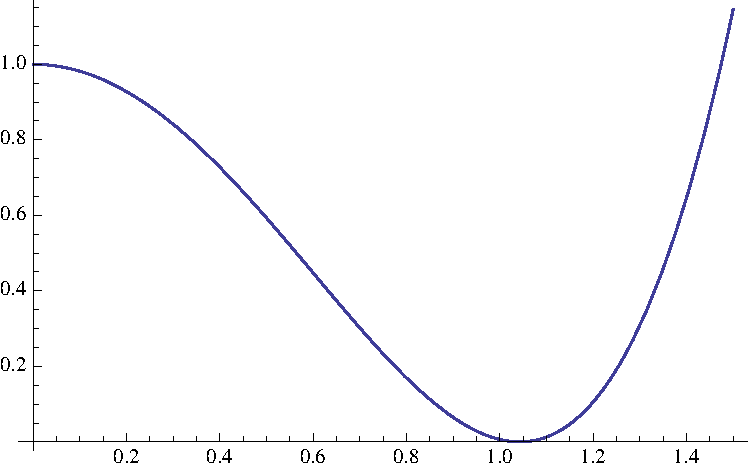
\includegraphics[width=0.7\textwidth]{optimizationplot}
\end{center}
\caption{A plot of $1+x^4 + y\p{\frac{x^4}{12} + x^2}$ with $y=-1.840265763084$ equal to its optimal value.  The zero near $x=1$ shows that $-y$ cannot be further increased without violating the positivity constraint.}
\label{fig:plot}
\end{figure}

\subsection{Checkpoints}

Every \texttt{checkpointInterval}, \SDPB\ saves a new checkpoint file with a \texttt{.ck} extension and backs up the old checkpoint file to a \texttt{.ck.bk} extension.  \SDPB\ also saves a checkpoint after termination, provided the option \texttt{--noFinalCheckpoint} is not specified.  

A checkpoint file encodes the values of $x,X,y,Y$.  If \SDPB\ detects an existing checkpoint file on startup, it will use those values of $x,X,y,Y$ as initial conditions in the solver.  Thus, \SDPB\ can be stopped and started at will without losing progress.

A typical workflow for long-running computations on shared machines is to specify a moderate \texttt{checkpointInterval} (e.g. one hour) and a somewhat larger \texttt{maxRuntime} (e.g. 12 hours).  \SDPB\ will terminate after 12 hours and can then be restarted without losing progress.  If \SDPB\ is killed prematurely, then at most 1 hour of progress will be lost.  This pattern of restarting gives other users chances to run their processes.  It can be sustained indefinitely, allowing extremely long computations.

\section{Attribution}

If you use \SDPB\ in work that results in publication, please cite \cite{DSD}. Depending on how \SDPB\ is used, the following sources might also be relevant:
\begin{itemize}
\item The first use of semidefinite programming in the bootstrap \cite{Poland:2011ey}.
\item The generalization of semidefinite programming methods to arbitrary
spacetime dimension \cite{Kos:2013tga}.
\item The generalization of semidefinite programming methods to arbitrary
systems of correlation functions \cite{Kos:2014bka}.
\end{itemize}

\section{Acknowledgements}

\SDPB\ Makes extensive use of \texttt{MPACK} \cite{MPACK}, the multiple precision linear algebra library written by Nakata Maho.  Several source files from \texttt{MPACK} are included in the \SDPB\ source tree (see the license at the top of those files). \SDPB\ uses Lee Thomason's \texttt{tinyxml2} library \cite{TINYXML2} for parsing.
The design of \SDPB\ was partially based on the solvers \texttt{SDPA} and \texttt{SDPA-GMP} \cite{SDPA,SDPA2,SDPAGMP}, without which this software would never have been written.

Thanks to Filip Kos, David Poland, and Alessandro Vichi for collaboration in developing semidefinite programming methods for the conformal bootstrap and assistance testing \SDPB.  Thanks to Amir Ali Ahmadi, Hande Benson, Pablo Parrilo, and Robert Vanderbei for advice and discussions about semidefinite programming.

\begin{thebibliography}{9}

\bibitem{DSD}
  David Simmons-Duffin,
  ``A Semidefinite Program Solver for the Conformal Bootstrap,"
  \href{http://arXiv.org}{arXiv:1502.xxxxx [hep-th]}.

%\cite{Poland:2011ey}
\bibitem{Poland:2011ey} 
  D.~Poland, D.~Simmons-Duffin and A.~Vichi,
  ``Carving Out the Space of 4D CFTs,''
  JHEP {\bf 1205}, 110 (2012)
  \href{http://arXiv.org/abs/1109.5176}{arXiv:1109.5176 [hep-th]}.
  %%CITATION = ARXIV:1109.5176;%%
  %71 citations counted in INSPIRE as of 01 Feb 2015
  
%\cite{Kos:2013tga}
\bibitem{Kos:2013tga} 
  F.~Kos, D.~Poland and D.~Simmons-Duffin,
  ``Bootstrapping the $O(N)$ vector models,''
  JHEP {\bf 1406}, 091 (2014)
  \href{http://arXiv.org/abs/1307.6856}{arXiv:1307.6856 [hep-th]}.
  %%CITATION = ARXIV:1307.6856;%%
  %29 citations counted in INSPIRE as of 01 Feb 2015

%\cite{Kos:2014bka}
\bibitem{Kos:2014bka} 
  F.~Kos, D.~Poland and D.~Simmons-Duffin,
  ``Bootstrapping Mixed Correlators in the 3D Ising Model,''
  JHEP {\bf 1411}, 109 (2014)
  \href{http://arXiv.org/abs/1406.4858}{arXiv:1406.4858 [hep-th]}.
  %%CITATION = ARXIV:1406.4858;%%
  %9 citations counted in INSPIRE as of 01 Feb 2015

\bibitem{SDPA}
  M. Yamashita, K. Fujisawa, M. Fukuda, K. Nakata, and M. Nakata,
  ``A high-performance software package for semidefinite programs: SDPA 7,''
   Research Report B-463, Dept. of Mathematical and Computing Science, Tokyo Institute of Technology, Tokyo, Japan (2010).

\bibitem{SDPA2}
  M. Yamashita, K. Fujisawa, and M. Kojima,
  ``Implementation and evaluation of SDPA 6.0 (SemiDefinite Programming Algorithm 6.0),''
  Optimization Methods and Software" 18 491-505 (2003).

\bibitem{SDPAGMP}
  M. Nakata,
  ``A numerical evaluation of highly accurate multiple-precision arithmetic version of semidefinite programming solver: SDPA-GMP, -QD and -DD.,''
  2010 IEEE International Symposium on Computer-Aided Control System Design (CACSD), 29-34 Sept 2010.

\bibitem{MPACK}
  M. Nakata,
  ``The MPACK (MBLAS/MLAPACK); a multiple precision arithmetic version of BLAS and LAPACK,''
  2010
  \href{http://mplapack.sourceforge.net/}{http://mplapack.sourceforge.net/}.

\bibitem{TINYXML2}
  L. Thomason,
  TinyXML2,
  \href{http://www.grinninglizard.com/tinyxml2docs/index.html}{http://www.grinninglizard.com/tinyxml2docs/index.html}

\end{thebibliography}

\end{document}